\documentclass[../thesis.tex]{subfiles}
\graphicspath{{\subfix{figs/ses_ling/}}}
\addbibresource{biblio.bib}
\begin{document}

\chapter{SES x language}
\label{ch:ses_ling}

\epigraph{
  This was not to say that Albertine had not already possessed [...] a quite
  adequate assortment  of those expressions which reveal at once that one's people are
  in easy circumstances, and which, year by year, a mother passes on to her daughter
  just as she bestows on her [...]
  %, gradually, as the girl grows up, on important occasions,
  her own jewels.
}{
  \epigraphcite{ProustGuermantesWay1927}
}

Language bounds individuals together just as much as it divides them. Upon reading the
last sentence, one may first think of inter-language boundaries: if two individuals
cannot understand each other's language, communication is effectively very limited. In
this work, however, we delve into intra-language differences: when people speak the same
language, but differently, which is also a strong source of social divides. Language
variation in a population is driven by many factors, among which the socio-economic
background of individuals is essential. As the sociologist Pierre Bourdieu put it,
individuals possess different quantities of ``linguistic capital''
\cite{BourdieuLanguageSymbolic2009}, which gives them more or less power both in the
political and economic spheres. \Ac{SES} and this linguistic
variation are thus mutually sustaining: one inherits a \ac{SES} along which comes a
linguistic capital that contributes --- among other things --- to constrain them to
their status of origin. Understanding the mechanisms that lead to this linguistic
segregation is therefore of great importance. 

A first step toward understanding is to quantify the phenomenon. It has already been
measured by the PISA reports of the OECD \cite{OECDWhereAll2019}, which survey, among
others, the reading proficiency of 15-year-olds in 79 countries. They consistently show
that students with lower socio-economic background tend to perform worse at this test.
While these confirm there is an issue to tackle, they are not extensive enough. They do
not test language production, and not the whole population, but only a sample of
students of a specific age. Alternative empirical works are thus needed. In that vein,
some past work has investigated the dependence on \ac{SES} of the frequency of a few markers
of non-standard language in France, as seen on Twitter
\cite{LevyAbitbolSocioeconomicDependencies2018}, showing the potential of this data
source for such an analysis.
% TODO: references! \cite{LabovSocialStratification1966,TrudgillSocialDifferentiation1974} trudgill: preference of non standard of working class men
% \cite{DavilaInevitabilityStandard2016} why should standard language be considered normal or correct, superior
% \cite{EagleNetworkDiversity2010} We find that the diversity of individuals’ relationships is strongly correlated with the economic development of communities.
% \cite{ChambersSociolinguisticTheory2007} there is link between linguistic variation and social factors
% \cite{EisensteinDiffusionLexical2014} Twitter for geographical variation of linguistic variables
% \cite{KretzschmarLanguageVariation2010} what is the "normal" variant depends on your social group who have different perceptions on language
% \cite{LaksWhyThere2013} In such a conception, communication is a leading force in the emergence and stabilization of human linguistic competence, both diachronically and synchronically. In this approach, variation and heterogeneity are to be seen as core factors in shaping language. Thus, as argued some 50 years ago by Weinreich, variation and heterogeneity are to be regarded as structurally functional, and as fundamental dimensions of language.
% \cite{KinzlerNativeLanguage2007} social groups are partly built and opposed based on language, and very early
% \cite{LazerComputationalSocial2009} potential of computational social science
% \cite{GaoComputationalSocioeconomics2019} social media like Twitter to link SES and different social behaviours like

In this work, we investigate this inter-dependence in the UK, by way of measuring how Twitter users abide by the rules of the standard variety of their language, which is the one taught at schools.

\section{A role of SES?}

\subsection{Twitter data analysis}
To do so, we analyse the Tweets of identified UK residents with LanguageTool, an
open-source grammar, style and spell checker. As the tool is implemented in 15
languages, our study can actually be replicated in other countries as well. It enables
us to compute the frequency at which these users make different categories of mistakes,
according to standard rules. To assign a \ac{SES} to these users, we determine their area of
residence from the geotags attached to their Tweets. The areas considered are
administrative areas with a typical population of ten thousand. For those, we have the
average annual net income of their residents from the census, which gives us a proxy for the
\ac{SES} of our Twitter users.

Our unit areas for the study are the \SI{7201}{} \acp{MSOA}, which are areas created for
the output of the UK census estimates. They host at least \SI{5000}{} and at most
\SI{15000}{} inhabitants, with a typical population of \SI{10000}{}. Their boundaries
can be downloaded from the Open Geography portal of the Office for National
Statistics\footnote{\url{https://geoportal.statistics.gov.uk/maps/msoa-dec-2011-boundaries-generalised-clipped-bgc-ew-v3}}.
In the following, we only keep cells in which we had sufficient text from Twitter. Our
criterion is set so that we keep cells with at least 15 resident users, each of whom
must have written at least 100 words. This leaves us with \SI{4879}{} \acp{MSOA} for our
analysis.

\subsection{SES x grammar mistakes correlations}
Focusing on grammar mistakes, we then find a significant, but weak correlation (Pearson
r equal to -0.25) between the net income and the average frequency of mistakes in all
areas of the country. We then focus on metropolitan areas because we expect them to host
more linguistic and socio-economic heterogeneity than their rural counterparts. We also
happen to have more data in these on both mobility and language production, due to the
fact that Twitter users tend to be more urban. We therefore consider the 8 largest
metropolitan areas in England, and find large differences between these areas, with
correlations ranging from -0.07 in Sheffield to -0.5 in Bristol.
\begin{figure}[hb]
\centering
  \includegraphics[width=\textwidth]{ses_x_grammar_corrs}
  \caption{Light blue \SI{95}{\percent} confidence interval for the regression estimate}
  \label{fig:ses_x_grammar_corrs}
\end{figure}



\subsection{The role of assortativity}
The 2018 net annual income for \acp{MSOA} of England and Wales was obtained from the census\footnote{\url{https://www.ons.gov.uk/employmentandlabourmarket/peopleinwork/earningsandworkinghours/datasets/smallareaincomeestimatesformiddlelayersuperoutputareasenglandandwales}}

To find out what could
make these cities so different in that regard, we measure the assortativity in the
mobility patterns of their residents \cite{HilmanSocioeconomicBiases2022}. We thus
determine how likely people from different socio-economic classes are to interact with
each other.

Excluding Tweets from their cell of residence. \ac{SES} classes are defined such that each class has roughly the same population. Since our proxy for \ac{SES} is the average income in every \ac{MSOA}, every resident of a cell will necessarily be assigned to the same class. Considering the cells in a given metropolitan area, we rank them by increasing average net income. We get their population from the census\footnote{\url{https://www.nomisweb.co.uk/census/2011/ks101uk}}, denoted $N_c$ for each cell $c$ in the following.
Set of cells less populated than $c$: $S_c = \left\{ c' \in C \mid N_{c'} < N_c \right\}$, 
\begin{equation}
  \mathcal{C}_c = n_{\mathcal{C}} \left\lceil \frac{\sum_{c' \in S_c} N_{c'}}{\sum_{c' \in C} N_{c'}} \right\rceil
\end{equation}
with $\left\lceil \cdot \right\rceil$ representing the ceil function and $n_{\mathcal{C}}$ the number of classes we wish to define. $m_{u, c}$ the number of trips made by user $u$ to cell $c$. 
\begin{equation}
  M_{i, j} = \frac{
      \sum_{u \in \mathcal{C}_i} \sum_{c \in \mathcal{C}_j} m_{u, c}
    }{
      \sum_{j \in \mathcal{C}_j} \sum_{u \in \mathcal{C}_i} \sum_{c \in \mathcal{C}_j} m_{u, c}
    }
\end{equation}
\begin{figure}[h]
\centering
  \includegraphics[width=\textwidth]{cities_SES_mobility}
  \caption{}
  \label{fig:cities_SES_mobility}
\end{figure}

What we find is a very clear correlation between this assortativity measured
at the city level, and the correlation between SES and the frequency of grammar
mistakes, as shown in Figure \ref{fig:cities_assort_vs_grammar_and_SES_corr}. This indicates that the more mixing in the
population, the less the frequency of mistakes is determined by the SES of origin.
\begin{figure}[hb]
\centering
  \includegraphics[width=\textwidth]{cities_assort_vs_grammar_and_SES_corr}
  \caption{}
  \label{fig:cities_assort_vs_grammar_and_SES_corr}
\end{figure}



\section{Model}

\subsection{Definition}
Having identified the importance of social mixing, we wish to understand the mechanisms
behind this effect with a simple model.
There are several effects we wish to consider, described below.
\begin{enumerate}[(i)]
  \item One of the two varieties of the language may be more prestigious than the other.
  This is for example the case of the standard form: it is taught at schools and spoken
  by the mainstream media and the public institutions \cite{DavilaInevitabilityStandard2016}.
  \item Even though one variety may be less prestigious, it might still be preferred by a
  part of the population that has some kind of cultural attachment to it. For instance,
  slang can be preferred by members of lower \ac{SES}, as using it might give them a
  sense of group identity \cite{LabovSocialStratification1966,TrudgillSocialDifferentiation1974}.
  \item We previously observed very different mixing patterns in UK metropolises.
  Indeed, mobility can be very heterogeneous, so it should be possible to plug in any
  mobility pattern into the model to be able to understand how different mixing may
  affect the dynamics of the linguistic varieties.
\end{enumerate}

It considers agent who can have one of two \ac{SES} classes, living in two separate
cells, and who can either speak standard, or not. The standard form has a higher
prestige $l_v$ because it is for instance preferred in schools and in the media. Then,
each \ac{SES} class has a preference for one form, the lower class 1 is attached to the
non-standard form with a factor $q_1$, and inversely the higher class 2 is attached to
the standard one with $q_2$. When either of these three parameters has a value above
$0.5$, it means there is a preference for the respective form. Then for instance, when
an agent of low \ac{SES} speaking non-standard interacts with another agent speaking
standard, they have a probability $l_v (1 - q_1)$ to start using the standard form as
well. The agents can move from their residence cell with a probability $m_{i,j}$ at each
step, which thus controls the mixing of the two populations. Figure
\ref{fig:model_diagram} provides a summary of the model.
\begin{figure}[hb]
\centering
  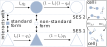
\includegraphics[width=\textwidth]{model_diagram}
  \caption{Diagram summarizing our agent-based model for the adoption of a linguistic variety. It features two \ac{SES} classes, represented by circles and triangles, which can speak one of two varieties of their language: the standard form (filled shapes) and the non-standard (empty shapes). Each agent has a cell of residence, and a mobility matrix with elements $m_{i, j}$ defines the probabilities for a resident of $i$ to be at different cells at each time step. After they have moved, for every agent, another agent is picked randomly for them to interact with, and if they happen to interact with an agent using the other variety, in function of their \ac{SES} class of origin they have different probabilities to adopt this variety. For instance, when a triangle (\ac{SES} 1) speaking non-standard interacts with another agent speaking standard, they have a probability equal to $l_v (1 - q_1)$ to adopt the standard form (transition represented in the bottom left).}
  \label{fig:model_diagram}
\end{figure}




\subsection{Properties of the model and behaviour in mean-field}
% fig with analytic result, stream plots, this kind of thing


\subsection{Simulating the model on a toy example}
We ran simulations with $200$ agents spread evenly between two SES classes,
with each class in its own residence cell. We set the standard form to be the more
prestigious one, agents with higher SES to be indifferent and ones with lower SES to be
more attached to the non-standard form. In Figure \ref{fig}(c), we show the result of
this simulation when we set a very low inter-cell mobility. For Figure \ref{fig}(d), the
mobility was greatly increased. We can see that the more the two populations mix, the
closer they are to using the two forms in the same proportions, reflecting what we
observed in the data.


\subsection{Simulating the model in real metropolitan areas}
This promising result calls for further investigation of the
model, and particularly how it would fare when initialised with the actual data that we
have in the metropolitan areas of England.


% fig with interesting simulation results: toy two cells into real populations?
\section{Discussion}



\end{document}
